\documentclass[12pt, a4paper]{report}
\usepackage[utf8]{inputenc}
\usepackage[english]{babel}
\usepackage[backend=biber,style=numeric]{biblatex}
\usepackage{csquotes}
\usepackage{graphicx}
\usepackage{epstopdf}
\usepackage{float}
\usepackage{moreverb}
\usepackage{hyperref}
\setlength{\parindent}{0em} 

\title{Übungsblatt 10}
\author{Thomas Samy Dafir}
\date{}
\hfuzz=10.0pt

\begin{document}
\maketitle

Alle Lösungen sind unter $buntmeise.cosy.sbg.ac.at$ verfügbar.

\section*{Aufgabe 1}
Grid Layout bietet eine einfache Möglichkeit, eine Seite oder Teile einer Seite auszurichten bzw. Tabellen abzulösen.\\
Verwendung:\\
\begin{itemize}
	\item Container element mit $display: grid$ oder $display: inline-grid$
	\item $grid-template-columns$ gibt die Breite der einzelnen Spalten an
	\item Zwischenräume zwischen den Zellen können mit $grid-column-gap$, $grid-row-gap$, $grid-gap$ gesetzt werden.
	\item $divs$ im container werden automatisch angeordnet, die Größe kann jedoch auch mittels $von-bis$ angegeben werden:\\
	$grid-column-start$\\
	$grid-column-end$\\
	$grid-row-start$\\
	$grid-row-end$\\
	Diese geben an, von welcher bis zu welcher Zellenbegrenzungslinie im Standard-Format eine Zelle reicht.
\end{itemize}

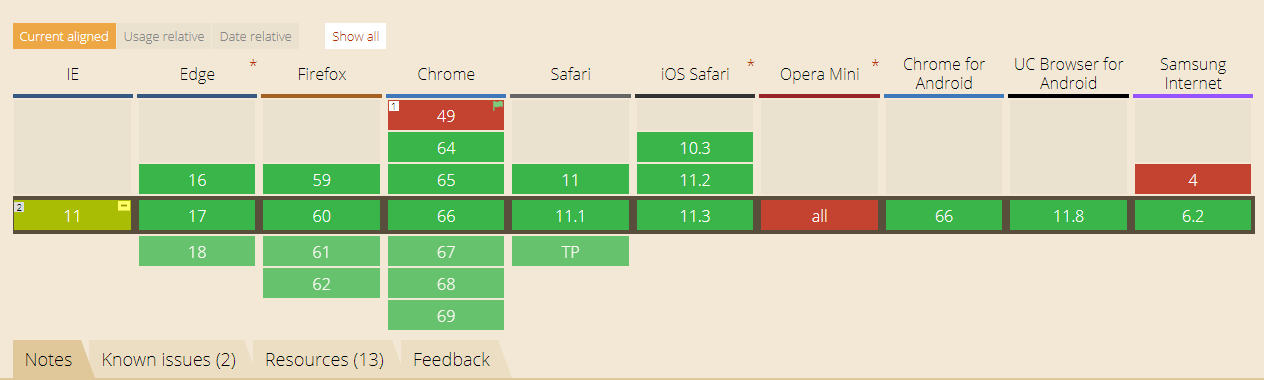
\includegraphics[width=\textwidth]{img/caniuse.png}

Quelle: https://www.w3schools.com/css/css\_grid.asp

\section*{Aufgabe 2}
Hierfür wurde eine einfache, rudimentär designte Website erstellt, die breakpoints und media-queries verwendet.
Die Site hat bei kleiner viewport size eine Top-Bar mit buttons, die an eine gegebene Stelle im Content verlinken.\\
Bei 700px Breite wechselt das Layout. Die Top-Bar wird durch eine Sidebar ersetzt. Der Content ist schmäler, erstreckt sich aber über die gesamte Höhe (20/80 Breitenverhältnis).\\
Diese beiden Ansichten werden durch das Media-Query $screen$ und entsprechende Breitenangabe erreicht. Es wurden bewusst sehr kräftige Farben gesetzt.\\
Im der Druckansicht wollen wir natürlich keinen Farbigen Hintergrund und auch die Leiste können wir uns sparen. Das wird erreicht, indem ein Media Query $@media print$ erstellt und mit CSS Regeln gefüllt wird. Content Breite und Höhe werden auf 100\% gesetzt die Leiste mit $display: none$ ausgeblendet und die Hintergrundfarben entfernt.

\section*{Aufgabe 3}
Autocomplete kann mit jquery sehr einfach verwendet werden.\\
Dazu werden jQuery, jQuery-UI und der zugehörigen jQuery-UI Style eingebunden und ein Array mit Werden, die für Autofill verwendet werden sollen definiert. Schließlich wird über einen Selektor das eingabefeld ausgewählt und die $autocomplete$ funktion aufgerufen. Dieser Funktion wird als Argument $source$ das definierte String-Array übergeben. Das Eingabefeld zeigt jetzt ab der Eingabe des ersten Buchstaben Vorschläge an.




\section*{Aufgabe 4}
-




















\end{document}
